  \let\negmedspace\undefined
\let\negthickspace\undefined
\documentclass[journal]{IEEEtran}
\usepackage[a5paper, margin=10mm, onecolumn]{geometry}
\usepackage{lmodern} % Ensure lmodern is loaded for pdflatex
\usepackage{tfrupee} % Include tfrupee package

\setlength{\headheight}{1cm} % Set the height of the header box
\setlength{\headsep}{0mm}     % Set the distance between the header box and the top of the text

\usepackage{gvv-book}
\usepackage{gvv}
\usepackage{cite}
\usepackage{amsmath,amssymb,amsfonts,amsthm}
\usepackage{algorithmic}
\usepackage{graphicx}
\usepackage{textcomp}
\usepackage{xcolor}
\usepackage{txfonts}
\usepackage{listings}
\usepackage{enumitem}
\usepackage{mathtools}
\usepackage{gensymb}
\usepackage{comment}
\usepackage[breaklinks=true]{hyperref}
\usepackage{tkz-euclide} 
\usepackage{listings}                                      
\def\inputGnumericTable{}                                 
\usepackage[latin1]{inputenc}                                
\usepackage{color}                                            
\usepackage{array}                                            
\usepackage{longtable}
\usepackage{multicol}
\usepackage{calc}                                             
\usepackage{multirow}                                         
\usepackage{hhline}                                           
\usepackage{ifthen}                                           
\usepackage{lscape}
\begin{document}

\bibliographystyle{IEEEtran}
\vspace{3cm}

\title{9.3.11}
\author{EE24BTECH11024 - G. Abhimanyu Koushik}
% \maketitle
% \newpage
% \bigskip
{\let\newpage\relax\maketitle}

\renewcommand{\thefigure}{\theenumi}
\renewcommand{\thetable}{\theenumi}
\setlength{\intextsep}{10pt} % Space between text and floats


\numberwithin{equation}{enumi}
\numberwithin{figure}{enumi}
\renewcommand{\thetable}{\theenumi}


\textbf{Question}:\newline
Solve the differential equation $\frac{d^2y}{dx^2} = y$ with initial conditions $y\brak{0} = 1$ and $y^{\prime}\brak{0} = 0$
\newline
\textbf{Solution: }
\newline
Theoritical Solution:\\
Laplace Transform definition\\
\begin{align}
	\mathcal{L}\brak{f\brak{t}} = \int_{0}^{\infty}e^{-st}f\brak{t}dt
\end{align}
Properties of Laplace tranform
\begin{align}
	\mathcal{L}\brak{y^{\prime\prime}} &= s^2\mathcal{L}\brak{y} -sy\brak{0}-y^\prime\brak{0}\\
	\mathcal{L}\brak{1} &= \frac{1}{s}\\
	\mathcal{L}\brak{cf\brak{t}} &= c\mathcal{L}\brak{f\brak{t}}\\
	\mathcal{L}\brak{f\brak{t}} = F\brak{s} &\implies \mathcal{L}\brak{e^{at}f\brak{t}} = F\brak{s-a}
\end{align}
Applying the properties to the given equation
\begin{align}
	y^{\prime\prime} - y &= 0\\
	\mathcal{L}\brak{y^{\prime\prime}} - \mathcal{L}\brak{y} &= 0\\
	s^2\mathcal{L}\brak{y} -sy\brak{0}-y^\prime\brak{0}-\mathcal{L}\brak{y} &= 0\\
\end{align}
Substituting the initial conditions gives
\begin{align}
	\brak{s^2-1}\mathcal{L}\brak{y}&= s\\
	\mathcal{L}\brak{y} &= \frac{s}{s^2 - 1}\\
	 \mathcal{L}\brak{y} &= \frac{1}{2\brak{s+1}}+\frac{1}{2\brak{s-1}}\\
	y &= \frac{1}{2}\brak{\mathcal{L}^{-1}\brak{\frac{1}{s+1}}+\mathcal{L}^{-1}\brak{\frac{1}{s-1}}}\\
	y &= \frac{1}{2}\brak{e^{-x}+e^{x}}u\brak{x}
\end{align}
The theoritical solution is 
\begin{align}
	f\brak{x} = \frac{1}{2}\brak{e^{-x}+e^{x}}u\brak{x}
\end{align}
We can arrive at a difference equation by applying Bilinear Z-transform on the Laplace equations. Take
\begin{align}
	s &= \frac{2}{T}\brak{\frac{1-z^{-1}}{1+z^{-1}}}
\end{align}
Here $T = h$
\begin{align}
	Y\brak{z} &= \frac{1}{2}\brak{\frac{1}{\frac{2}{T}\brak{\frac{1-z^{-1}}{1+z^{-1}}}+1}+\frac{1}{\frac{2}{T}\brak{\frac{1-z^{-1}}{1+z^{-1}}}-1}}\\
	Y\brak{z} &= \frac{1}{2}\brak{\frac{T\brak{1+z^{-1}}}{2\brak{1-z^{-1}}+T\brak{1+z^{-1}}}+\frac{T\brak{1+z^{-1}}}{2\brak{1-z^{-1}}-T\brak{1+z^{-1}}}}\\
	Y\brak{z} &= \frac{1}{2}\brak{\frac{T\brak{1+z^{-1}}}{\brak{T-2}z^{-1}+\brak{T+2}} - \frac{T\brak{1+z^{-1}}}{\brak{T+2}z^{-1}+\brak{T-2}}}\\
	\alpha_1 &= -\frac{T-2}{T+2}\\
	\alpha_2 &= -\frac{T+2}{T-2}\\ 
	Y\brak{z} &= \frac{T}{2\brak{T+2}}\brak{\frac{1}{1-\alpha_1z^{-1}}+\frac{z^{-1}}{1-\alpha_1z^{-1}}}-\frac{T}{2\brak{T-2}}\brak{\frac{1}{1-\alpha_2z^{-1}}+\frac{z^{-1}}{1-\alpha_2z^{-1}}}
\end{align}
The radius of convergence of $\frac{1}{1-\alpha_1z^{-1}}$ and $\frac{z^{-1}}{1-\alpha_1z^{-1}}$ is $\abs{z}>\abs{\alpha_1}$ and radius of convergence of $\frac{1}{1-\alpha_2z^{-1}}$ and $\frac{z^{-1}}{1-\alpha_2z^{-1}}$ is $\abs{z}>\abs{\alpha_2}$\\
The radius of convergence of $Y\brak{z}$ is $max\brak{\abs{\alpha_1},\abs{\alpha_2}}$\newline
Applying the inverse Z-transform with some rearrangement gives
\begin{align}
	\brak{1-\alpha_1z^{-1}}\brak{1-\alpha_2z^{-1}}Y\brak{z} = \frac{T}{2}\brak{1+z^{-1}}\brak{\frac{1-\alpha_2z^{-1}}{T+2}-\frac{1-\alpha_1z^{-1}}{T-2}}\\
	\brak{1-\brak{\alpha_1+\alpha_2}z^{-1}+z^{-2}}Y\brak{z} = \frac{T}{2}\brak{\frac{1-\brak{\alpha_2-1}z^{-1}-\alpha_2z^{-2}}{T+2}}\nonumber \\
  \qquad -\frac{T}{2}\brak{\frac{1-\brak{\alpha_1-1}z^{-1}-\alpha_1z^{-2}}{T-2}}\\
	z^2Y\brak{z}-z\brak{\alpha_1+\alpha_2}Y\brak{z}+Y\brak{z} = \frac{T}{2}\brak{\brak{\frac{z^2-\brak{\alpha_2-1}z-\alpha_2}{T+2}}-\brak{\frac{z^2-\brak{\alpha_1-1}z-\alpha_1}{T-2}}}\\
	z^2Y\brak{z}-z\brak{\alpha_1+\alpha_2}Y\brak{z}+Y\brak{z} -z^2y\sbrak{0} -zy\sbrak{1} -z\brak{\alpha_1+\alpha_2}y\sbrak{0}\nonumber
\end{align}
\begin{align}
  \qquad+z^2y\sbrak{0}+zy\sbrak{1}+z\brak{\alpha_1+\alpha_2}y\sbrak{0} = \frac{T}{2}\brak{\brak{\frac{z^2-\brak{\alpha_2-1}z-\alpha_2}{T+2}}-\brak{\frac{z^2-\brak{\alpha_1-1}z-\alpha_1}{T-2}}}\\
  y_{n+2}-\brak{\alpha_1+\alpha_2}y_{n+1}+y_n+\delta\sbrak{n+2}y\sbrak{0}+\delta\sbrak{n+1}\brak{y\sbrak{1}+\brak{\alpha_1+\alpha_2}y\sbrak{0}} = \nonumber \\
  \qquad\frac{T}{2}\brak{\delta\sbrak{n+2}\brak{\frac{1}{T+2}-\frac{1}{T-2}}-\delta\sbrak{n+1}\brak{\frac{\alpha_1-1}{T-2}+\frac{\alpha_2-1}{T+2}}+\delta\sbrak{n}\brak{\frac{\alpha_1}{T-2}-\frac{\alpha_2}{T+2}}}
\end{align}
Since $n\ge 0$, $\delta\sbrak{n+2} = 0$ and $\delta\sbrak{n+1} = 0$
\begin{align}
	 y_{n+2}-\brak{\alpha_1+\alpha_2}y_{n+1}+y_n = \frac{T}{2}\brak{\frac{\alpha_1}{T-2}-\frac{\alpha_2}{T+2}}\delta\sbrak{n}
\end{align}
As $y\sbrak{0} = 1$ from initial condition and
\begin{align}
y\sbrak{1}=y\brak{0} + hy^\prime\brak{0}\\
\end{align}
Hence $n\ge 2$ which gives the difference equation as
\begin{align}
	y_{n+2} = \brak{\alpha_1+\alpha_2}y_{n+1} - y_n
\end{align}
Computational Solution:\newline
The given differential equation is
\begin{align}
	y^{\prime\prime} - y = 0
\end{align}
Let
\begin{align}
	y^\prime = y_1\\
	y = y_2
\end{align}
Then
\begin{align}
	\frac{dy_1}{dx} &= y_2\\
	\frac{dy_2}{dx} &= y_1\\
	\int_{y_{1,k}}^{y_{1,k+1}}dy_1 &= \int_{x_k}^{x_{k+1}}y_2dx\\
	\int_{y_{2,k}}^{y_{2,k+1}}dy_2 &= \int_{x_k}^{x_{k+1}}y_1dx
\end{align}
Discretizing the steps using trapezoidal rule gives us
\begin{align}
	y_{1,k+1} - y_{1,k} = \frac{h}{2}\brak{y_{2,k}+y_{2,k+1}}\\
	y_{2,k+1} - y_{2,k} = \frac{h}{2}\brak{y_{1,k}+y_{1,k+1}}
\end{align}
Then solving for $y_{1,k+1}$ and $y_{2,k+1}$ in terms of $y_{1,k}$, $y_{2,k}$ and $h$ will help us to calculate the value of function at $x_{k+1}$
\begin{align}
	y_{1,k+1} = y_{1,k} + \frac{h}{2}\brak{y_{2,k}+\brak{y_{2,k}+\frac{h}{2}\brak{y_{1,k}+y_{1,k+1}}}}\\
	y_{1,k+1} = y_{1,k}\brak{1+\frac{h^2}{4}} + y_{2,k}h + y_{1,k+1}\brak{\frac{h^2}{4}}\\
	y_{1,k+1}\brak{1-\frac{h^2}{4}} = y_{1,k}\brak{1+\frac{h^2}{4}} + y_{2,k}h\\
	y_{1,k+1} = \frac{\brak{y_{1,k}}\brak{4+h^2}+4h\brak{y_{2,k}}}{4-h^2}
\end{align}
Similarly
\begin{align}
y_{2,k+1} = \frac{\brak{y_{2,k}}\brak{4+h^2}+4h\brak{y_{1,k}}}{4-h^2}
\end{align}
The difference equations are
\begin{align}
y_{1,k+1} = \frac{\brak{y_{1,k}}\brak{4+h^2}+4h\brak{y_{2,k}}}{4-h^2}\\
y_{2,k+1} = \frac{\brak{y_{2,k}}\brak{4+h^2}+4h\brak{y_{1,k}}}{4-h^2}
\end{align}
Using the above formula, recording the value of $y$ at each value of $x_{k} = x_0 + kh$ and taking $y\brak{0} = 1$ and $y^\prime\brak{0}=0$ and plotting gives
\begin{figure}[h!]
   \centering
   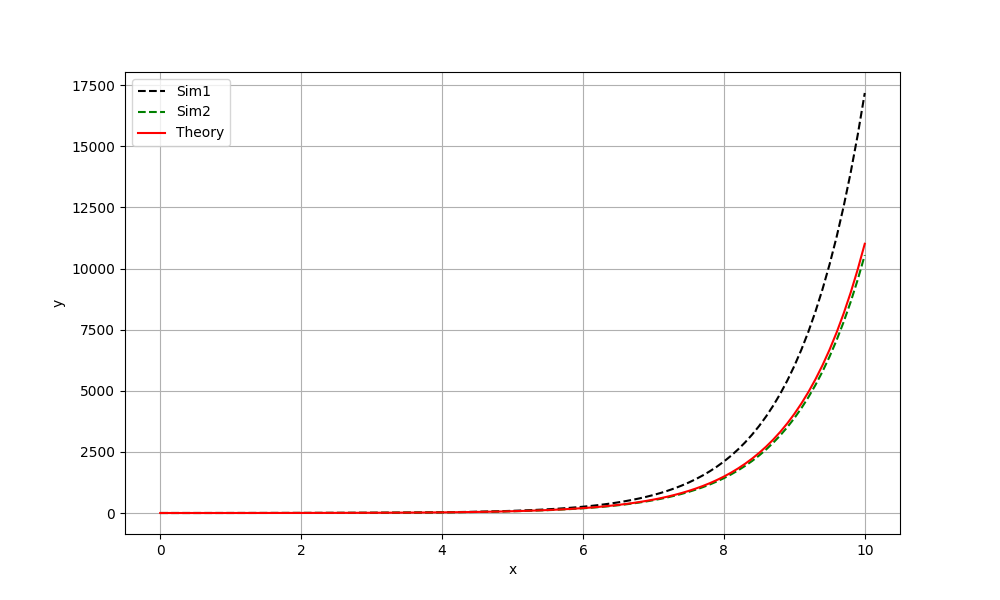
\includegraphics[width=\columnwidth]{figs/fig.png}
   \caption{Comparison between the Theoritical solution and Computational solutions, Red is theory, Black line is derived from difference equation from Trapezoidal method, while Green line is from Z-transform while taking stepsize to be 0.1}
   \label{stemplot}
\end{figure}
\end{document}  
